% 原书 p.237–p.244（PDF p.245–p.252）
% 第 9 章 9.2 节：$A_\infty$-代数与势函数

% >>> p245
\section{$A_\infty$-代数与势函数（$A_\infty$-algebra and Potential Function）}

\begin{keytakeaways}
\begin{itemize}
  \item 几何图像：$A_\infty$-代数把伪全纯曲线模空间中「冒泡」与「断裂」的复杂行为打包为
        一条代数恒等式 $(\sum_k\hat m_k)^2=0$；对拉格朗日子流形取相对
        Gromov--Witten 不变量即可得到这种结构。
  \item 数学工具：分次代数、bar 复形 $B(C)$、$A_\infty$-关系、Koszul 符号、界定上链
        （bounding cochain）、弱 Maurer--Cartan 方程、Novikov 环
        $\Lambda^{\mathbf{k},\Gamma_\omega}$。
  \item 本节结论：定理 9.2.1（Fukaya--Oh--Ohta--Ono：$(C^*(L),\{m_k\})$ 是
        $A_\infty$-代数）、势函数 $\mathfrak{PO}_L$ 的定义 9.2.2 及其在辛环面流形上的
        显式公式 (9.18)；据此给出定理 9.1.2 的证明。
\end{itemize}
\end{keytakeaways}

$A_\infty$-代数结构出现在辛几何中，乍看也许令人惊讶，但它实际上是一种联系几何与代数的
自然代数结构。它开启了现代辛几何的大门，并提供了精确描述相应模空间中伪全纯曲线
「冒泡」（bubbling）或「断裂」（breaking）复杂行为的途径。本节我们将介绍
$A_\infty$-代数结构，并展示它如何帮助构造一个辛不变量（称为\textbf{势函数}，
potential function），用以在辛同胚意义下区分拉格朗日子流形。关于这一代数结构的完整
发展（特别是它与辛几何的深刻联系），见 [88] 的第一部分。

固定一个含幺环 $R$（乘法单位元为 $1$）以及一个分次 $R$-代数
$C=\oplus_{k\in\N}C^k$，其中第一项是环 $R$（对应 $k=0$）。

\begin{wdefn}{9.2.1}
  一个分次 $R$-代数 $C$ 称为 \textbf{$A_\infty$-代数}，如果它允许一列
  $R$-同态 $\{m_k\colon C^{\otimes k}\to C\}_{k\in\N}$（包括 $k=0$ 时的
  $m_0\colon R\to C$），满足如下定义的「微分关系」。考虑 $C$ 的 \textbf{bar 复形}
  \begin{equation*}
    B(C):=\bigoplus_{k=0}^\infty C^{\otimes k}
    =R\oplus C\oplus C^{\otimes2}\oplus C^{\otimes3}\oplus\cdots.
  \end{equation*}
  先用下式定义映射 $\hat m_k$，从而把 $m_k$ 延拓到 $B(C)$ 上：
  \begin{equation*}
    \hat m_k(x_1\otimes\cdots\otimes x_n)
    :=\sum_{i=1}^{n-k+1}(-1)^*x_1\otimes\cdots\otimes
    m_k(x_i\otimes\cdots\otimes x_{i+k-1})\otimes x_{i+k}\otimes\cdots\otimes x_n,
  \end{equation*}
  其中 $x_1\otimes\cdots\otimes x_n\in C^{\otimes n}$ 是任意单项式，$n\geqslant k$
  （若 $n<k$ 则定义为 $0$）。这里
  $*=\deg(x_1)+\cdots+\deg(x_{i-1})+(i-1)$。然后把 $\hat m_k$ 按线性性延拓到
  $B(C)$ 上。$B(C)$ 上所需的「微分关系」为
  \begin{equation}\tag{9.11}
    \Bigl(\sum_{k=0}^\infty\hat m_k\Bigr)^2=0.
  \end{equation}
\end{wdefn}
% [Tutor Note: 易错预警——$\hat m_k$ 中的符号 $(-1)^*$ 同时包含 Koszul 符号与
% 「移位」因子 $(i-1)$：前者来自把 $m_k$ 越过 $x_1,\cdots,x_{i-1}$，后者是
% $A_\infty$-代数作为「带移位的分次代数」所固有的（不同文献对是否显式写出 $(i-1)$
% 约定不同，等价于把 $C$ 整体平移一次）。因此同一关系在不同教材中可能相差
% $(-1)^{\deg}$ 因子；本书始终采用上述约定，后文 (9.12)、(9.13) 等计算均以此为准。
% 若在 $\Z/2\Z$ 上工作，则一切符号消失。]

% >>> p246
\begin{wrem}{9.2.1}
  特别地，当 $k=0$ 时，由于 $C^0=R$，$m_0$ 由 $m_0(1)$ 唯一确定。此外，按定义
  \begin{equation*}
    \hat m_0(x_1\otimes\cdots\otimes x_n)
    =m_0(1)\otimes x_1\otimes\cdots\otimes x_n
    \pm x_1\otimes m_0(1)\otimes\cdots\otimes x_n\pm\cdots
    \pm x_1\otimes\cdots\otimes x_n\otimes m_0(1),
  \end{equation*}
  其中 $m_0(1)$ 插入到每一对相邻的 $x_i\otimes x_{i+1}$ 之间（包括起始位置与末尾
  位置）。更具体地说，若 $n=1$，则
  $\hat m_0(x)=m_0(1)\otimes x+(-1)^{\deg(x)+1}x\otimes m_0(1)$。
\end{wrem}

\begin{wrem}{9.2.2}
  可以把 $A_\infty$-代数看成经典链复形（见例 9.2.2）的推广版本；很可能在不久的将来，
  它会在数学的许多其他分支中成为常识。
\end{wrem}

为简单起见，人们常常在 $R=\Z/2\Z$ 上工作，从而忽略定义 9.2.1 中 $\hat m_k$ 的符号
$(-1)^*$。这样许多验证都会简化。

\begin{wexam}{9.2.1}
  把微分关系 (9.11) $\bigl(\sum_{k=0}^\infty\hat m_k\bigr)^2=0$ 的一些初等情形写出来
  是有启发性的。
  对 $1\in R$，关系 (9.11) 作用在 $1$ 上等价于
  \begin{equation}\tag{9.12}
  \begin{aligned}
    &(\hat m_0+\hat m_1+\cdots)(\hat m_0+\hat m_1+\cdots)(1)\\
    &\quad=(\hat m_0+\hat m_1+\cdots)\bigl(m_0(1)\bigr)\\
    &\quad=m_0(1)\otimes m_0(1)+m_0(1)\otimes m_0(1)+m_1(m_0(1))
      =m_1(m_0(1))=0.
  \end{aligned}
  \end{equation}
  对任意 $x\in C$，关系 (9.11) 作用在 $x$ 上给出
  \begin{equation}\tag{9.13}
  \begin{aligned}
    &(\hat m_0+\hat m_1+\hat m_2+\cdots)
      (\hat m_0+\hat m_1+\hat m_2+\cdots)(x)\\
    &\quad=(\hat m_0+\hat m_1+\hat m_2+\cdots)
      \bigl(m_0(1)\otimes x+x\otimes m_0(1)+m_1(x)\bigr)\\
    &\quad=m_1(m_1(x))+m_2(m_0(1)\otimes x)+m_2(x\otimes m_0(1))=0.
  \end{aligned}
  \end{equation}
  % [Tutor Note: 原文疑误/约定——(9.12) 与 (9.13) 实际上是在「忽略符号」（即
  % $R=\Z/2\Z$）的约定下写出的：在带符号约定下，$\hat m_0(m_0(1))$ 的两项
  % $m_0(1)\otimes m_0(1)$ 相差一个 $(-1)$ 而相消（因为
  % $\hat m_0(x)=m_0(1)\otimes x+(-1)^{\deg x+1}x\otimes m_0(1)$，此处 $\deg m_0(1)=0$），
  % (9.13) 中 $m_1(m_0(1)\otimes x)$ 与 $m_1(x\otimes m_0(1))$ 的符号也由 $\deg x$ 决定。
  % 作者把两项都写成「$+$」，读者应理解为模 2 计算；结论
  % $m_1(m_0(1))=0$ 与 $m_1(m_1(x))=0$（在 $m_0=0$ 时）本身与约定无关。]

  若把 $m_1$ 视为 $C$ 的「微分」（于是 $(C,m_1)$ 看起来像一个链复形），则由 (9.12)
  知 $m_0(1)$ 是闭的。然而 (9.13) 表明 $(C,m_1)$ 一般并不是链复形（即 $m_1^2=0$
  未必成立），其障碍由 $m_0(1)\neq0$ 给出。\hfill$\square$
\end{wexam}

\begin{wexam}{9.2.2}
  回忆\textbf{微分分次代数}（differential graded algebra，DGA）是一对
  $(C=\oplus C^k,\dd)$，其中 $C$ 是分次代数（乘积记为 $\cdot$），$\dd$ 是微分，且
  这两种结构满足 Leibniz 法则（见下面的练习）。它可以看作一个 $A_\infty$-代数，其中
  $m_0=0$，$m_1=\dd$，$m_2=\cdot$（代数乘法），且 $m_{k\geqslant3}=0$。
  \hfill$\square$
\end{wexam}

% >>> p247
\begin{wexer}{9.2.1}
  \begin{enumerate}[label=(\alph*)]
    \item 对微分分次代数 $(C,\dd)$，Leibniz 法则
      $\dd(a\cdot b)=\dd a\cdot b\pm a\cdot\dd b$（或
      $m_1(m_2(a\otimes b))=m_2(m_1(a)\otimes b)\pm m_2(a\otimes m_1(b))$）
      是 $A_\infty$-代数微分方程 (9.11) 的一个子关系。
    \item 给定 $A_\infty$-代数 $(C,\{m_k\}_{k=0}^\infty)$，设 $m_{k\geqslant3}=0$。
      证明运算 $m_2$ 的结合性，即
      $m_2(m_2((x\otimes y)\otimes z))=m_2(m_2(x\otimes(y\otimes z)))$。
  \end{enumerate}
\end{wexer}

\begin{wque}{9.2.1}
  给定 $A_\infty$-代数 $(C,\{m_k\}_{k=0}^\infty)$，其中 $m_0(1)\neq0$，如何以 $C$
  为基础得到一个链复形？换言之，如何把 $\{m_k\}$ 修改为 $\{m'_k\}$，使得
  $m'_0(1)=0$ 且 $(C,\{m'_k\}_{k=0}^\infty)$ 仍是 $A_\infty$-代数？
\end{wque}

让我们先在一个容易的情形中试一试。对给定的 $(C,\{m_k\}_{k=0}^\infty)$，取元素
$e\in C^1$，满足
\begin{equation*}
  m_2(x,e)=\pm m_2(e,x)=x\quad\text{和}\quad m_k(\cdots,e,\cdots)=0
\end{equation*}
对任何其它正整数 $k$ 成立。若这样的 $e$ 存在，则容易由 (9.13) 验证：若
$m_0(1)=\lambda e$（其中 $\lambda\in R$），则 $m_1\circ m_1=0$。这样的元素
$e\in C^1$ 通常称为 $A_\infty$-代数 $(C,\{m_k\}_{k=0}^\infty)$ 的\textbf{单位}
（unit）。

对一般情形，为简化讨论，设 $m_{k\geqslant3}=0$ 且 $R=\Z/2\Z$。那么标准做法是按如下
方式「形变」$m_k$。取 $b\in C$ 使得
\begin{equation}\tag{9.14}
  \sum_{k=0}^\infty m_k(b^{\otimes k})
  =m_0(1)+m_1(b)+m_2(b\otimes b)=0.
\end{equation}
把 $m_k$ 形变为
\begin{equation}\tag{9.15}
  m_k^b(x_1\otimes\cdots\otimes x_k)
  =\sum_{l_0,\cdots,l_k\geqslant0}
  m_{k+\sum_{i=0}^k l_i}
  \bigl(b^{\otimes l_1}\otimes x_1\otimes b^{\otimes l_2}\otimes x_2\otimes\cdots
  \otimes x_k\otimes b^{\otimes l_k}\bigr).
\end{equation}
% [Tutor Note: 原文疑误——(9.15) 右端求和指标为 $l_0,\cdots,l_k$（共 $k+1$ 个），
% 但被求值的单项式中只出现 $b^{\otimes l_1},\cdots,b^{\otimes l_k}$（共 $k$ 个），
% 指标 $l_0$ 未出现。按形变公式的通常含义，$k$ 个输入之间及两端应有 $k+1$ 段 $b$
% 因子，故应写成
% $b^{\otimes l_0}\otimes x_1\otimes b^{\otimes l_1}\otimes\cdots\otimes x_k
% \otimes b^{\otimes l_k}$（下标整体平移），或把求和指标改为 $l_1,\cdots,l_{k+1}$。
% 译文按原文照译，详见 qsg/notes/review_ch09a.md。]

更具体地说，对我们的情形，由 (9.14)，
\begin{equation*}
\begin{aligned}
  m_0^b(1)&=m_0(1)+m_1(b)+m_2(b\otimes b)+0=0,\\
  m_1^b(x)&=m_1(x)+m_2(b\otimes x)+m_2(x\otimes b),\\
  m_2^b(x_1\otimes x_2)&=m_2(x_1\otimes x_2).
\end{aligned}
\end{equation*}
下面验证 $(C,\{m_k^b\}_{k=0}^\infty)$ 仍是 $A_\infty$-代数。为简化叙述，我们只对
$x\in C$ 验证 (9.11)。由于 $m_0^b(1)=0$ 且 $m_{k\geqslant3}=0$，(9.11) 在
$x\in C$ 上的条件转化为
\begin{equation}\tag{9.16}
\begin{aligned}
  (\hat m_1^b+\hat m_2^b)^2(x)
  &=\hat m_1^b\bigl(\hat m_1^b(x)\bigr)\\
  &=\hat m_1^b\bigl(m_1(x)+m_2(b\otimes x)+m_2(x\otimes b)\bigr)\\
  &=m_1(m_1(x))+m_1\bigl(m_2(b\otimes x)+m_2(x\otimes b)\bigr)\\
  &\quad+m_2(b\otimes m_1(x))+m_2(b\otimes m_2(b\otimes x))
    +m_2(m_2(b\otimes x)\otimes b)\\
  &\quad+m_2(m_1(x)\otimes b)+m_2(m_2(b\otimes x)\otimes b)
    +m_2(m_2(x\otimes b)\otimes b).
\end{aligned}
\end{equation}
% [Tutor Note: 原文疑误——上式末两行中的 $m_2(m_2(b\otimes x)\otimes b)$ 出现两次，
% 而按 $\hat m_1^b$ 的展开应有一项为 $m_2(b\otimes m_2(x\otimes b))$；疑原文重复/漏项。
% 此外本式与下一段的改写式逐项核对也有出入。此两处均照原文译出，详见
% qsg/notes/review_ch09a.md。]

% >>> p248
由 $m_1$ 的 Leibniz 法则，有
\begin{equation*}
  m_1\bigl(m_2(b\otimes x)+m_2(x\otimes b)\bigr)
  =m_2(m_1(b)\otimes x)+m_2(b\otimes m_1(x))
  +m_2(m_1(x)\otimes b)+m_2(x\otimes m_1(b)).
\end{equation*}
于是 (9.16) 可改写为
\begin{equation*}
\begin{aligned}
  &m_1(m_1(x))+m_2(b\otimes m_1(x))+m_2(m_1(x)\otimes b)+m_2(m_1(b)\otimes x)\\
  &\qquad+m_2(b\otimes m_1(x))+m_2(b\otimes m_2(b\otimes x))
    +m_2(x\otimes m_1(b))+m_2(m_2(x\otimes b)\otimes b)\\
  &=m_1(m_1(x))+m_2(m_0(1)\otimes x)+m_2(m_2(b\otimes b)\otimes x)
    +m_2(b\otimes m_2(b\otimes x))\\
  &\qquad+m_2(x\otimes m_0(1))+m_2(x\otimes m_2(b\otimes b))
    +m_2(m_2(x\otimes b)\otimes b)=0,
\end{aligned}
\end{equation*}
这里我们用 (9.13) 与 (9.14) 得出最后一步（$=0$）。此外，由于 $m_0^b(1)=0$，我们
得到链复形 $(C,m_1^b)$。

注意，到目前为止我们还没有确认满足 (9.14) 的 $b$ 一定存在。一般地，从 $m_k$ 到
$m_k^b$ 的形变归结为能否求解如下非线性方程：
\begin{equation*}
\tag*{(9.16)}
  m_0(1)+m_1(b)+m_2(b\otimes b)+\cdots=0.
\end{equation*}
这个方程称为 \textbf{Maurer--Cartan 方程}，其任一解 $b$ 称为\textbf{界定上链}
（bounding cochain）。
% [Tutor Note: 原文疑误——原书在此处再次标号 (9.16)，与上页（p.239 末）的 (9.16)
% 重复。为忠实呈现原文且避免 LaTeX 标签重复，此式在译文中用 \tag*{(9.16)} 排出，
% 显示样式与 (9.16) 一致。详见 qsg/notes/review_ch09a.md。]

\begin{wrem}{9.2.3}
  可以用类似方式验证：若 $b$ 满足
  \begin{equation*}
    m_0(1)+m_1(b)+m_2(b,b)+\cdots=\lambda(b)\cdot e
  \end{equation*}
  其中 $\lambda(b)\in R$（依赖于 $b$），$e\in C^1$ 是单位，则同样的形变仍然有效。
  更多细节见 [88]。这样的方程称为\textbf{弱 Maurer--Cartan 方程}，其解 $b$ 称为
  \textbf{弱界定上链}（weak bounding cochain）。若 $b$ 变动，则 $\lambda$ 可视为
  一个 $R$-值函数。
\end{wrem}
% [Tutor Note: 原文疑误——上式左端第二项写作 $m_2(b,b)$，与 $m_2$ 的定义域
% $C\otimes C$ 不符，应为 $m_2(b\otimes b)$（对照 (9.16) 与 $M_{\mathrm{weak}}(L)$
% 的定义）。译文按原文照写为 $m_2(b,b)$，详见 qsg/notes/review_ch09a.md。]

回到我们的故事：在辛几何中我们在哪里遇到 $A_\infty$-代数？下面的例子演示了一种情形。

\begin{wexam}{9.2.3}
  给定辛流形 $(M,\omega)$ 与拉格朗日子流形 $L\subset(M,\omega)$，我们将进行
  Gromov--Witten 不变量的一个「相对」版本。这里只给出概略性的描述，更严格的发展
  可参见 [88] 第一部分第 3 章。

  回忆 Gromov--Witten 不变量经由稳定映射的模空间 $\mathcal M_k(A,J)$ 来计数从曲面
  （球面 $(S^2,j)$）到辛流形 $(M,\omega,J)$ 的 $J$-全纯曲线（球面），其中 $A$ 是
  拓扑约束，$k$ 是标记点的个数。Gromov--Witten 不变量的相对版本将计数
  $J$-全纯圆盘
  \begin{equation*}
    u\colon(\mathbb{D}^2,\partial\mathbb{D}^2,j)\to(M,L,J),
  \end{equation*}
  其模空间为稳定映射的模空间 $\mathcal M_k(\beta,J)$，其中 $\beta\in\pi_2(M,L)$。
  这里按记号约定，要求 $u$ 把边界 $\partial\mathbb{D}^2$ 映入拉格朗日子流形 $L$。
  这样的 $J$-全纯圆盘可用图 9.3 示意。
\end{wexam}
% [Tutor Note: 含糊点拨——例 9.2.3 中「相对 Gromov--Witten 不变量」的严格定义需要
% 对模空间 $\mathcal M_k(\beta,J)$ 取虚拟基本类（或 Kuranishi 结构），并验证边界
% 赋值映射 $\mathrm{ev}_0$ 与 Poincaré 对偶的横截性；这里的「概略描述」省略了这些
% 技术细节，作者把严格处理留给 [88]。阅读时注意 $\beta$ 是相对于 $(M,L)$ 的第二个
% 相对同伦群元素，Maslov 指标 $\mu(\beta)$ 在其上有定义。]

% >>> p249
沿边界 $\partial\mathbb{D}^2$ 指定 $k$ 个标记点。考虑上闭链
$a_1,\cdots,a_k\in C^*(L)$（其中 $C^*(L)$ 视为奇异上链复形），要求
$u(z_i)\in\mathrm{PD}_L(a_i)$ 且 $[u]=\beta\in\pi_2(M,L)$，就可定义并计算相对
Gromov--Witten 不变量，记作
$^{\mathrm{rel}}\mathrm{GW}_{\beta,k}(a_1,\cdots,a_k)$。这里 Poincaré 对偶
$\mathrm{PD}_L$ 是在 $L$ 本身上进行的。

\begin{figure}[htbp]
  \centering
  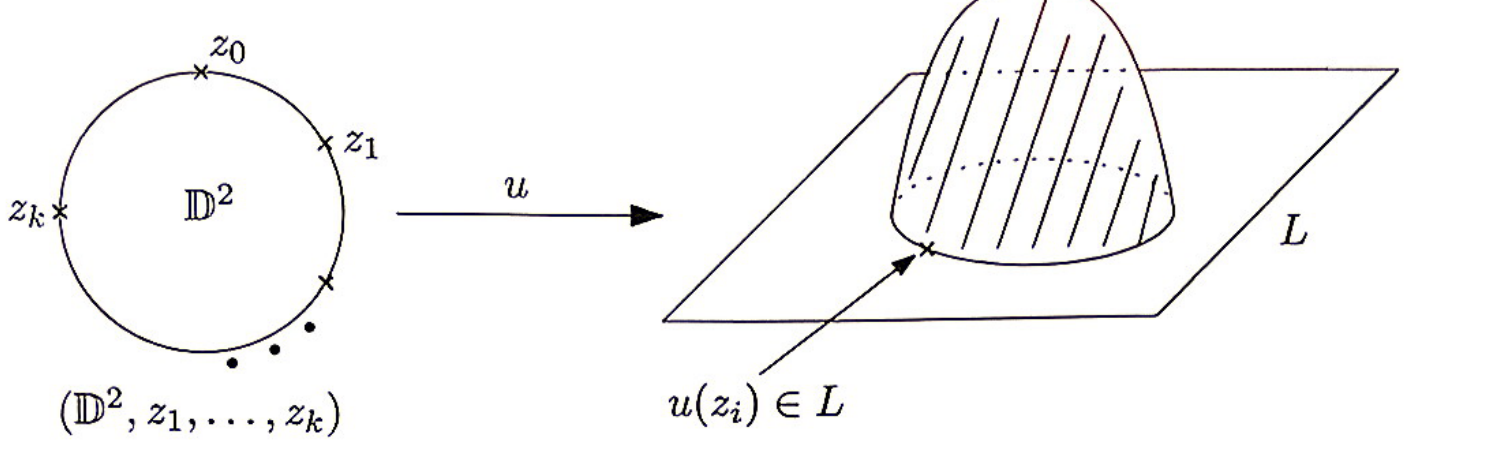
\includegraphics[width=0.8\linewidth]{figures/fig_p249_1.png}
  \caption*{图 9.3\quad 带 $k$ 个标记点的 $J$-全纯圆盘（原书 p.241, Figure 9.3；
  PDF p.249）}
\end{figure}

为借助 $^{\mathrm{rel}}\mathrm{GW}_{\beta,k}$ 构造 $A_\infty$-代数，我们需要目标取为
$C^*(L)$（而不是标量），使得
$m_k\colon C^*(L)\otimes\cdots\otimes C^*(L)\to C^*(L)$ 有定义。为此，考虑
$\mathcal M_{k+1}(\beta,J)$，其中增加了一个额外标记点 $z_0$。于是对每个
$\beta\in\pi_2(M,L)$ 与 $a_1,\cdots,a_k\in C^*(L)$，定义
\begin{equation*}
  m_{k,\beta}(a_1,\cdots,a_k)
  :=\mathrm{PD}_L\Bigl((\mathrm{ev}_0)_*\bigl(\mathcal M_{k+1}(\beta,J)
  \cap\mathrm{PD}_L(a_1)\cap\cdots\cap\mathrm{PD}_L(a_k)\bigr)\Bigr).
\end{equation*}
然后按如下方式定义 $m_k$（系数取自 8.1 节引入的 Novikov 环
$\Lambda^{\mathbf{k},\Gamma_\omega}$）：
\begin{equation}\tag{9.17}
  m_k(a_1,\cdots,a_k):=\sum_{\substack{\beta\in\pi_2(M,L)\\\mu(\beta)=2}}
  m_{k,\beta}(a_1,\cdots,a_k)T^{\omega(\beta)},
\end{equation}
其中 $\mu(\beta)$ 是 $\beta$ 的 Maslov 指标（依据定义 7.3.1 定义），
$\omega(\beta)\geqslant0$ 是 $\beta$ 的 $\omega$-面积。通常把
$\Lambda^{\mathbf{k},\Gamma_\omega}$ 换为
$\Lambda^{\mathbf{k},\Gamma_\omega}_{\geqslant0}$，其中
\begin{equation*}
  \Lambda^{\mathbf{k},\Gamma_\omega}_{\geqslant0}
  =\Bigl\{\sum a_iT^{\lambda_i}\Bigm|\lambda_i\geqslant0,\ \lambda_i\to\infty\Bigr\}
\end{equation*}
表示 Novikov 环（域）$\Lambda^{\mathbf{k},\Gamma_\omega}$ 的「非负部分」。注意按定义
$m_k$ 是 $\Lambda^{\mathbf{k},\Gamma_\omega}_{\geqslant0}$-模同态。下面这个结果是
拉格朗日子流形最基本性质之一，它基于同调方法。

\begin{wthm}{9.2.1}（Fukaya--Oh--Ohta--Ono）
  对任意拉格朗日子流形 $L\subset(M,\omega)$，上述定义的
  $(C^*(L),\{m_k\}_{k=0}^\infty)$ 是 $A_\infty$-代数。
\end{wthm}

粗略地说，来自 (9.11) 的「微分关系」给出了一个代数打包，它编码了模空间
$\mathcal M_{k+1}(\beta,J)$ 中 $J$-全纯圆盘所有可能的「冒泡」（参见例 8.3.1）。
\hfill$\square$

在上面的例子中，按照文献中的标准约定，取
$R=\Lambda^{\mathbf{k},\Gamma_\omega}_{\geqslant0}$ 作为 $A_\infty$-代数
$(C^*(L),\{m_k\}_{k=0}^\infty)$ 的环。于是可以显式写出

% >>> p250
映射 $m_0\colon\Lambda^{\mathbf{k},\Gamma_\omega}_{\geqslant0}\to C^*(L)$ 如下：
\begin{equation*}
  m_0(1)=\sum_{\substack{\beta\in\pi_2(M,L)\\\mu(\beta)=2}}
  m_{0,\beta}(1)T^{\omega(\beta)}
  =\sum_{\substack{\beta\in\pi_2(M,L)\\\mu(\beta)=2}}
  \mathrm{PD}\bigl(\mathrm{ev}_*(\mathcal M_1(\beta,J))\bigr)T^{\omega(\beta)}.
\end{equation*}
同时，记
\begin{equation*}
  \mathcal M_{\mathrm{weak}}(L)
  :=\bigl\{b\in C^*(L)\bigm|m_0(1)+m_1(b)+m_2(b\otimes b)+\cdots
  =\lambda(b)\cdot\mathbf{1}_L\bigr\},
\end{equation*}
它包含所有关于 $\mathbf{1}_L=\mathrm{PD}_L([L])$ 的弱界定上链。由注 9.2.3，可以
考虑取 $\Lambda^{\mathbf{k},\Gamma_\omega}_{\geqslant0}$ 值的函数 $\lambda$，它是由
拉格朗日子流形 $L$ 构造的辛不变量。

给定拉格朗日子流形 $L\subset(M,\omega)$，若
$\mathcal M_{\mathrm{weak}}(L)\neq\varnothing$，则对任意
$b\in\mathcal M_{\mathrm{weak}}(L)$，由上面的讨论可把 (9.17) 中的 $m_k$ 形变为
$m_k^b$，使得上同调群 $H^*(C^*(L),m_1^b)$ 有定义。这个群称为 $L$ 的
\textbf{拉格朗日 Floer 上同调}。

\begin{wdefn}{9.2.2}
  给定辛流形 $(M,\omega)$ 的拉格朗日子流形 $L$，其中
  $\mathcal M_{\mathrm{weak}}(L)\neq\varnothing$，则函数
  $\lambda\colon\mathcal M_{\mathrm{weak}}(L)\to
  \Lambda^{\mathbf{k},\Gamma_\omega}_{\geqslant0}$ 称为 $L$ 的\textbf{势函数}
  （potential function），记作 $\mathfrak{PO}_L$。
\end{wdefn}

一般地，计算 $\mathcal M_{\mathrm{weak}}(L)$ 或函数 $\lambda$ 是不可能的。下面是一类
特殊的辛流形，其中 $\mathcal M_{\mathrm{weak}}(L)$ 与 $\lambda$ 均可计算。回忆
定义 2.5.2：辛环面流形（symplectic toric manifold）$(M^{2n},\omega)$ 是一个闭辛流形，
它允许 $n$-环面 $\mathbb{T}^n$ 的某个群作用。辛环面流形的一个关键特征是：它允许一个
矩映射 $\mu\colon(M^{2n},\omega)\to\R^n$，该映射由 $\mathbb{T}^n$ 的李代数的线性
无关分量构造（更多细节见 2.5 节）。$\mu$ 在 $\R^n$ 中的像称为 $(M^{2n},\omega)$ 的
\textbf{矩像}（moment image）。

\whead{事实}{9.2.1}（Fukaya--Oh--Ohta--Ono）\quad
给定辛环面流形 $(M^{2n},\omega)$，其矩像为 $\Omega\subset\R^n$。则对任意点
$x\in\Omega$ 及其纤维（作为 $n$ 维拉格朗日环面）$\mu^{-1}(x)\subset M$，有
\begin{equation*}
  \mathcal M_{\mathrm{weak}}\bigl(\mu^{-1}(x)\bigr)
  \supset H^1\bigl(\mu^{-1}(x);
  \Lambda^{\mathbf{k},\Gamma_\omega}_{\geqslant0}\bigr).
\end{equation*}
特别地，$\mathcal M_{\mathrm{weak}}(\mu^{-1}(x))\neq\varnothing$（因为
$H^1(\mu^{-1}(x);\Lambda^{\mathbf{k},\Gamma_\omega}_{\geqslant0})\neq0$）。
\par\medskip
% [Tutor Note: 含糊点拨——事实 9.2.1 是 Fukaya--Oh--Ohta--Ono 的经典结论：对辛环面
% 流形，矩映射纤维 $\mu^{-1}(x)$ 是拉格朗日环面，其上的弱界定上链可取为
% $H^1(\mu^{-1}(x);\Lambda)$ 中的元素（几何上对应环面上的调和 $1$-形式、即
% $\dd\theta_i$ 的常系数组合，配合 Novikov 系数），相应的 $J$-全纯圆盘 Maslov 指标
% 为 $2$。注意包含方向是 $\supset$：弱界定上链的集合更大，$H^1$ 只是其中一部分；
% 用 $H^1$ 中的元素已足以定义势函数。]

对辛环面流形 $(M,\omega)$（外加 $(M,\omega)$ 是单调的，即满足条件 (8.1)），关于
纤维拉格朗日环面 $\mu^{-1}(x)$ 的势函数，即
\begin{equation*}
  \mathfrak{PO}_{\mu^{-1}(x)}\colon H^1\bigl(\mu^{-1}(x);
  \Lambda^{\mathbf{k},\Gamma_\omega}_{\geqslant0}\bigr)
  \to\Lambda^{\mathbf{k},\Gamma_\omega}_{\geqslant0},
\end{equation*}
对矩像 $\Omega$ 中任意 $x$，可按相当显式的方式计算：
\begin{enumerate}[label=(\arabic*)]
  \item 把 $H^1(\mu^{-1}(x);\Lambda^{\mathbf{k},\Gamma_\omega}_{\geqslant0})$
    与 $(\Lambda^{\mathbf{k},\Gamma_\omega}_{\geqslant0})^n$ 在坐标
    $y=(y_1,\cdots,y_n)$ 下等同起来。
\end{enumerate}

% >>> p251
\begin{enumerate}[label=(\arabic*),start=2]
  \item 由定理 2.5.1，矩像 $\Omega$ 是一个凸包。特别地，$\partial\Omega$ 由若干超平面
    组成。每个超平面由方程
    \begin{equation*}
      \langle x,v\rangle-c=0\quad\text{其中}\ x\in\R^n
    \end{equation*}
    给出，其中 $v$ 表示 $\partial\Omega$ 的内向单位法向量，$c$ 是某个常数。把所有
    超平面标为 $l_1=0,\cdots,l_m=0$，其中每个 $l_i\colon\R^n\to\R$ 由单位法向量
    $v_i$ 与某个相应的截距 $c_i$ 唯一确定（$i=1,\cdots,m$）。下面的图 9.4 给出了
    一个例子。
\end{enumerate}

\begin{figure}[htbp]
  \centering
  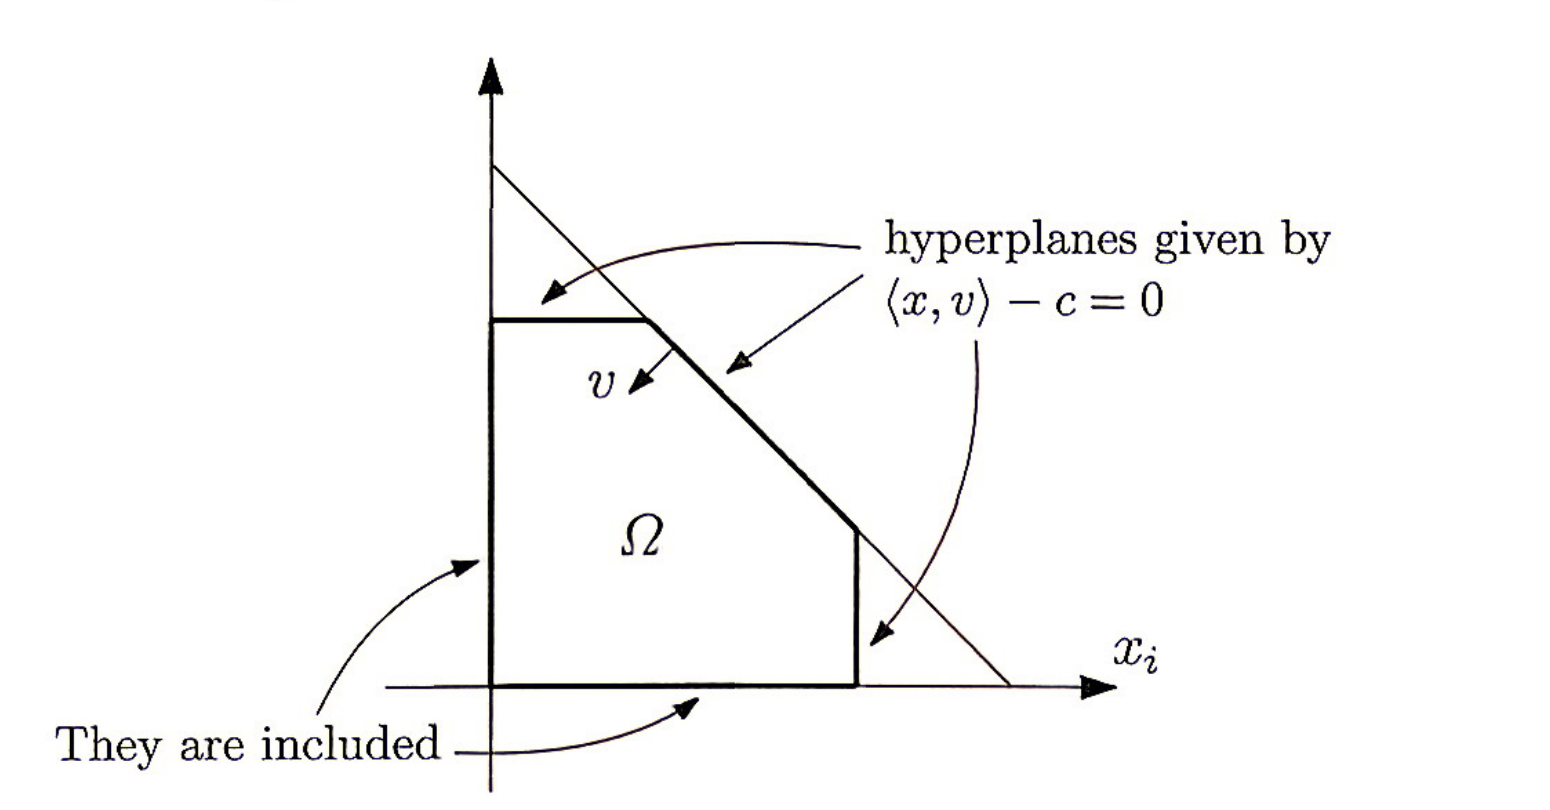
\includegraphics[width=0.62\linewidth]{figures/fig_p251_1.png}
  \caption*{图 9.4\quad 由方程确定的超平面（原书 p.243, Figure 9.4；PDF p.251）}
\end{figure}

\begin{enumerate}[label=(\arabic*),start=3]
  \item 势函数由下式给出：
    \begin{equation}\tag{9.18}
      \mathfrak{PO}_{\mu^{-1}(x)}(y)
      =\sum_{i=1}^m\ee^{\langle v_i,y\rangle}T^{l_i(x)}
    \end{equation}
    对任意 $y\in H^1(\mu^{-1}(x);
    \Lambda^{\mathbf{k},\Gamma_\omega}_{\geqslant0})$ 成立（见上面 (1)）。
\end{enumerate}
% [Tutor Note: 易错预警——(9.18) 中的 $l_i(x)$ 是第 $i$ 个超平面方程的左端在 $x$
% 处的取值（按 (2) 中的约定 $l_i(x)=\langle x,v_i\rangle-c_i$），而 $v_i$ 是
% \emph{内}向法向量，故在 $\Omega$ 内部 $l_i(x)\geqslant0$，从而 $T^{l_i(x)}$ 属于
% $\Lambda^{\mathbf{k},\Gamma_\omega}_{\geqslant0}$。若把 $v_i$ 取成外法向量，
% 指数上的符号会整体改变，势函数也随之为另一个函数；这是核对 (9.18) 与
% 例 9.2.4 时最容易出错之处。]

\begin{wexam}{9.2.4}
  取辛环面流形 $(M,\omega)=(S^2\times S^2,\omega_{\mathrm{prod}})$。由例 2.5.4，
  其矩像 $\Omega$ 是 $\R^2_{\geqslant0}$ 中的正方形（在坐标 $(x_1,x_2)$ 下），
  如图 9.5 所示。显然有四个超平面构成边界 $\partial\Omega$。相应的函数
  $l_1,\cdots,l_4$ 如下：
  \begin{equation*}
  \begin{aligned}
    l_1((x_1,x_2))&=\langle x,(0,-1)\rangle+1,&\quad
    l_2((x_1,x_2))&=\langle x,(-1,0)\rangle+1,\\
    l_3((x_1,x_2))&=\langle x,(0,1)\rangle,&\quad
    l_4((x_1,x_2))&=\langle x,(1,0)\rangle.
  \end{aligned}
  \end{equation*}
  注意按定义，对点 $(0.5,0.5)\in\Omega$，原像
  $\mu^{-1}((0.5,0.5))$ 恰是 9.1 节构造的 Clifford 环面
  $\mathbb{T}_{\mathrm{Clifford}}$。应用公式 (9.18)，
  \begin{equation*}
    \mathfrak{PO}_{\mathbb{T}_{\mathrm{Clifford}}}(y_1,y_2)
    =\ee^{-y_2}T^{1/2}+\ee^{-y_1}T^{1/2}+\ee^{y_2}T^{1/2}+\ee^{y_1}T^{1/2}.
  \end{equation*}
\end{wexam}

% >>> p252
\begin{figure}[htbp]
  \centering
  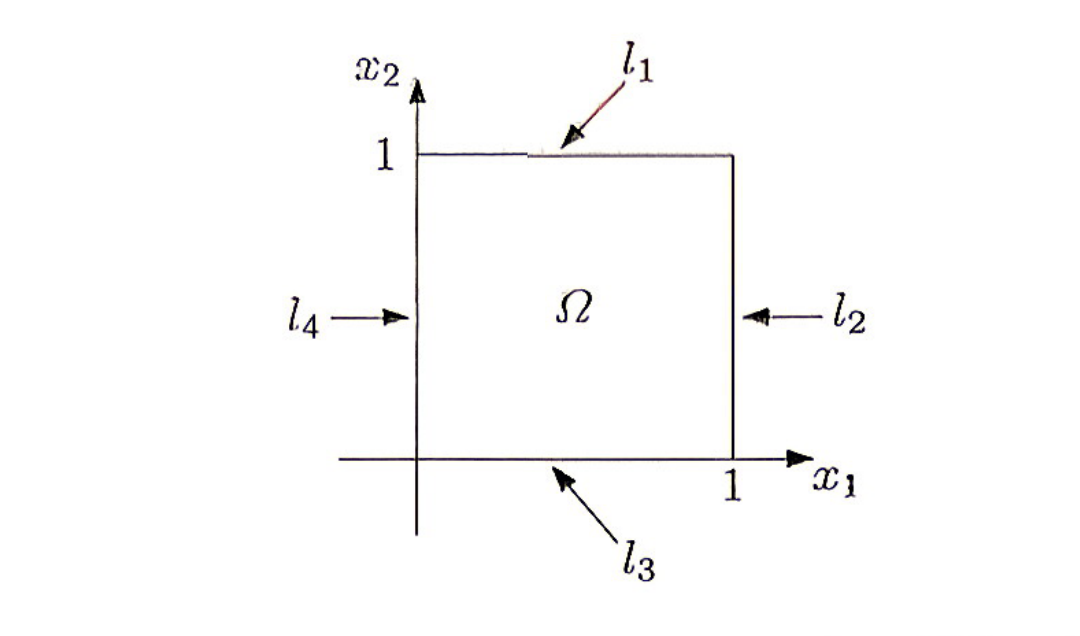
\includegraphics[width=0.6\linewidth]{figures/fig_p252_1.png}
  \caption*{图 9.5\quad $(S^2\times S^2,\omega_{\mathrm{prod}})$ 的矩像 $\Omega$ 中的
  超平面（原书 p.244, Figure 9.5；PDF p.252）}
\end{figure}

令 $z_1=\ee^{y_1}$、$z_2=\ee^{y_2}$ 并在 $T=1$ 处取值，我们有
\begin{equation}\tag{9.19}
  \mathfrak{PO}_{\mathbb{T}_{\mathrm{Clifford}}}(z_1,z_2)\big|_{T=1}
  =z_1+z_2+\frac1{z_1}+\frac1{z_2},
\end{equation}
作为 $\mathbb{T}_{\mathrm{Clifford}}$ 的一个辛不变量。\hfill$\square$

\begin{wexer}{9.2.2}
  回忆 $(\CP^2,\omega_{\mathrm{FS}})$ 是辛环面流形 $X_\Omega$，其矩像 $\Omega$ 是
  $\R^2$ 中的标准二维单纯形，即
  $\Omega=\{(x_1,x_2)\in\R^2_{\geqslant0}\mid x_1+x_2\leqslant1\}$。对任意
  $x\in\operatorname{int}(\Omega)$，计算势函数
  $\mathfrak{PO}_{\mu^{-1}(x)}$。这里我们只关注
  $\mathfrak{PO}_{\mu^{-1}(x)}$ 的定义域
  $H^1(\mu^{-1}(x);\Lambda^{\mathbf{k},\Gamma_\omega}_{\geqslant0})
  \simeq(\Lambda^{\mathbf{k},\Gamma_\omega}_{\geqslant0})^2$。
\end{wexer}

\whead{事实}{9.2.2}（[20] 中的推论 5.13）\quad
对 9.1 节构造的 $(S^2\times S^2,\omega_{\mathrm{prod}})$ 中的拉格朗日环面
$\mathbb{T}_{\mathrm{CS}}$，其势函数 $\mathfrak{PO}$ 计算如下：
\begin{equation*}
  \mathfrak{PO}_{\mathbb{T}_{\mathrm{CS}}}(z_1,z_2)\big|_{T=1}
  =z_1+\frac{(1+z_2)^2}{z_1z_2}.
\end{equation*}
\par\medskip

于是可以很快证明定理 9.1.2。

\begin{wproof}[定理 9.1.2 的证明]
  由于 $\mathfrak{PO}$ 是辛不变量，所需结论来自例 9.2.4 中的 (9.19) 与事实 9.2.2。
\end{wproof}
% [Tutor Note: 含糊点拨——原文此处只以「$\mathfrak{PO}$ 是辛不变量」一句带过，略去了
% 严格的比较步骤：$z_i$ 的选取依赖于矩像坐标与 $H^1$ 的基，两个环面的势函数应在
% 单项式变量代换 $z_i\mapsto T^{\lambda_i}z_i$ 以及 $H^1$ 基的整系数线性变换下比较；
% 需验证不存在这样的代换把 (9.19) 的 $z_1+z_2+z_1^{-1}+z_2^{-1}$ 与事实 9.2.2 的
% $z_1+(1+z_2)^2/(z_1z_2)$ 互变。这一步在原文中被省略，读者可自行补全。]
